\chapter{Projetos relacionados}

\section{Sistemas existentes no mercado}

\subsection{Sistemas comerciais}
Atualmente, já existem sistemas comerciais de automação residencial --- a maioria deles atuando de maneira mais forte do mercado norte-americano. Alguns dos sistemas mais populares nessa linha são o Amazon Echo e o Google Home.

O Amazon Echo\footnote{http://www.amazon.com/oc/echo/} consiste em um \textit{smart speaker} (alto-falante inteligente) conectado ao assistente pessoal Alexa, também da Amazon, que é capaz de entender comandos de voz. Inicialmente, funcionava como uma maneira de encomendar produtos, mas, atualmente, além de ser assistente pessoal, também é capaz de controlar diversos \textit{smart devices} da casa, como um \textit{hub} de automação residencial. Uma limitação deste produto é dependência de conexão \textit{wireless} de Internet, não sendo capaz de operar em nenhum nível sem ela.

Uma característica interessante do Alexa é a possibilidade de adição de novas \textit{skills} (habilidades) por desenvolvedores, que possuem acesso a uma API pública, documentada e disponibilizada \textit{online}. Dessa forma, seu \textit{skillset} é passível de grande expansão e personalização. Além disso, o serviço de voz desse sistema, conhecido como Alexa Voice Service, pode ser utilizado por qualquer dispositivo que contenha microfone e alto falante, e que consiga conectar-se a ele pela Internet.

O Google Home\footnote{https://madeby.google.com/home/} é similar ao Amazon Echo em alguns aspectos, sendo também um \textit{smart speaker}, que surgiu como expansão do aplicativo para smartphones Google Now, um assistente pessoal. Atualmente existe também como aplicativo para smartphones. Não é possível o desenvolvimento de módulos e expansões ao Google Home por desenvolvedores desvinculados à Google, porém ela trabalha diretamente com outras marcas e produtos para o estabelecimento de parcerias, de forma que o Google Home também consiga funcionar como \textit{hub} de automação residencial.

\subsection{Sistemas \emph{open-source}}
Também existem diversos projetos \emph{open-source} sobre o tema, cujas documentações estão disponíveis publicamente na Internet. Alguns desses projetos, analisados para o desenvolvimento do Hedwig, foram o OpenHAB e o Home Assistant.

O OpenHAB\footnote{http://www.openhab.org/} possui como objetivo principal o estabelecimento de uma plataforma de integração, capaz de solucionar o problema atual de haver diversos dispositivos em uma residência que não são capazes de se comunicar, devido à falta de uma linguagem comum para a troca informações. Por ser independente de hardware específico, é extremamente flexível e personalizável, porém isso implica em maior complexidade para o usuário no momento de sua instalação. O OpenHAB apresenta interface para o usuário em cliente web e aplicativos nativos para iOS e Android.

O Home Assistant\footnote{https://github.com/home-assistant/home-assistant} é uma plataforma de automação residencial capaz de controlar e monitorar os diversos dispositivos em uma casa, oferecendo uma plataforma web para o controle do sistema pelo usuário. O controlador local é implementado em Python, e recomenda-se instalá-lo em um Raspberry Pi. Possui diversas integrações já estabelecidas, com sistemas e serviços como o próprio Amazon Echo, Google Cast, IFTTT, Digital Ocean, entre outros, mas possibilita também a criação de novos componentes pelos próprios usuários. A personalização pelos usuários é feita por meio de um arquivo de configuração no formato YAML.

Os dois projetos apresentam como maior dificuldade a necessidade do usuário possuir conhecimentos técnicos para utilizá-los.

\section{Projeto HomeSky}

O Projeto HomeSky \cite{homeSky} é um Trabalho de Conclusão de Curso desenvolvido por alunos de Engenharia de Computação na Escola Politécnica da Universidade de São Paulo. Com o objetivo de fomentar iniciativas de desenvolvimento na área de casas inteligentes, o trabalho focou-se na criação do Rainfall, um protocolo em código aberto a nível de aplicação para ser usado na coordenação de uma rede de sensores. Isso permitiria aos desenvolvedores ter uma maior flexibilidade em seus projetos, visto que muitas das soluções existentes são proprietárias. Por fim, também foi realizada a implementação de um algoritmo de aprendizado de máquina capaz de controlar a iluminação.

\begin{figure}[H]
	\centering
	\caption{Camadas da arquitetura usada no Projeto HomeSky. As camadas em verde correspondem às bibliotecas desenvolvidas no trabalho.}
  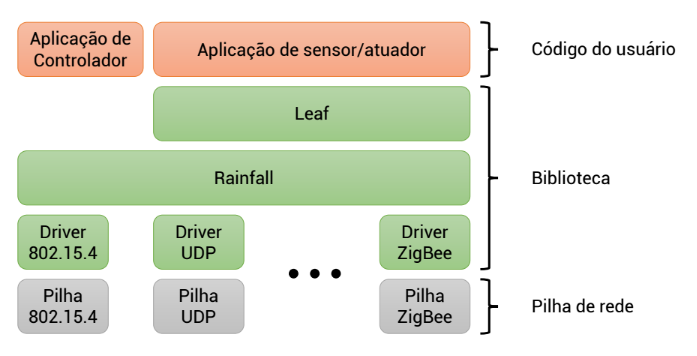
\includegraphics[width=0.8\textwidth]{arquiteturaHomeSky}
	\caption*{Fonte: \cite{homeSky}}
\label{fig:arquiteturaHomeSky}
\end{figure}

No desenvolvimento do protocolo Rainfall, foram consideradas algumas hipóteses simplificadoras a respeito da conectividade e da segurança. O protocolo não trata de forma especial a fase de conexão à rede, considerando que todos os nós já estão conectados a ela, e também considera que todos os protocolos adjacentes são confiáveis, delegando as implementações de mecanismos de reconhecimento de entrega e retransmissão ao desenvolvedor. Quanto à segurança, assume-se que a infraestrutura seja segura e que nenhum nó conectado à rede tenha comportamento mal intencionado, como por exemplo espionar mensagens destinadas a outros nós ou fingir ser o controlador.
